\subsection{Paradigms and Idioms}
The paradigms and idioms is the mid level of software abstraction in our taxonomy. This level requires the suggested code satisfy all the previous levels of abstractions and use common paradigms and language idioms in its suggestions, these include common practices of performing a task in a programming language. 
For example, considering the task of sorting operation on a list of numbers. To satisfy this level of abstraction, \cct{} should suggest a syntactically correct list sorting code, using idioms like best way to swap items in a list~(line 8 in fig~\ref{fig:idioms}) instead of using another temp variable~(shown in fig~\ref{fig:correctness}). 

The main goal of this level in the taxonomy is for \cct{} to be able to detect and use the commonly used practices occur in public code in its code suggestions to a problem.
Figure~\ref{fig:idioms} shows the example and the suggestions from \cct{} at this abstraction level.

\begin{figure}[hbt!]
    \centering
    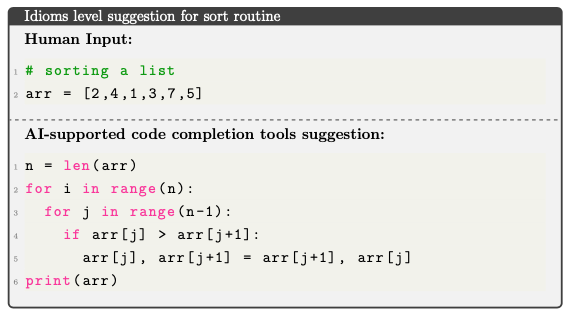
\includegraphics[width=\linewidth]{Figures/idioms.png}
    \caption{\cct{} paradigms and idioms level suggestions}
    \label{fig:idioms}
\end{figure}

The capabilities required by \cct{} to satisfy this level of abstraction are as follows:
\begin{enumerate}
    \item Identify common patterns like paradigms and language idioms in public code~(training data).
    \item Use paradigms and language idioms in suggesting solutions for a problem.
    \item Satisfy requirements of all the levels below paradigms and idioms in our taxonomy.
\end{enumerate}

% \begin{tcolorbox}[title=Idioms level suggestion for sort routine,boxsep=.15mm]
%     %https://tex.stackexchange.com/questions/337909/tcolorbox-tcbline-style
% \textbf{Human Input:}
% \begin{lstlisting}[language={Python}]
% # sorting a list
% arr = [2,4,1,3,7,5]
% \end{lstlisting}
% \tcbline
% \textbf{\cct{} suggestion:}
% \begin{lstlisting}[language={Python}]
% n = len(arr)
% for i in range(n):
% 	for j in range(n-1):
% 		if arr[j] > arr[j+1]:
% 			arr[j], arr[j+1] = arr[j+1], arr[j]
% print(arr)
% \end{lstlisting}
% \end{tcolorbox}